%-------------------------------------------------------------------------
%
% Master-2 NPAC 
%
% NPAC Lab Projects: template article
%
% The final article should not have more than 4 pages
% you are not allowed to modify fonts, page size and margins.
% Anything after the end of the 4th page will be ignored.
%
%-------------------------------------------------------------------------
%
% To compile your article with LaTeX, do this on the terminal:
%   
%        pdflatex article-template.tex
%
% This will produce a PDF file. Figures may be PDF files, images, etc.
% If you have PS/EPS figures convert them first in PDF files.
%
% You may need to compile twice to get the references properly set.
% 
%-------------------------------------------------------------------------
% 
%
\documentclass[final,12pt]{article}
%
\usepackage{npac}
\usepackage{amsmath}
\usepackage{url}
\usepackage{graphicx}
\usepackage{color}
\usepackage[T1]{fontenc}
\usepackage[french]{babel}
\usepackage[utf8]{inputenc}

%
\begin{document}
%
\title{Manipulation de suites P-récursives avec SageMath}
\author{Mathis \textsc{Carisntan} \& Aurélien \textsc{Lamoureux} \\ {\small sous la responsabilité de Marc \textsc{Mezzarobba}}}
%
\date{09/03/2017}

\maketitle
%
\begin{abstract}
    Ce rapport présente le travail que nous avons effectué au cours de ce projet.
    Nous présentons dans un premier temps ce que sont les suites P-récursives,
    ainsi que l'outil SageMath. Puis nous expliquons les motivations de ce projet.
    Enfin, nous détaillons les choix et détails de l'implémentation que nous avons réalisé,
    avant de discuter des limites de celle-ci et des possibles améliorations.
\end{abstract}

\section{Introduction}
    \label{intro}
    Nous nous intéressons

\section{Experimental Setup}

The text goes here. It could be a good idea to give an overview of your
experimental setup for instance...

If you want to cite an article of the bibliography, you should do
\cite{ipn-web} or \cite{Boh}. And if you want to cite a previous
section, the introduction for instance: the details can be found in
Sec. \ref{intro}. Don't forget to label the sections you want to
cite. 

You may do the same to refer to a figure: like see fig.~\ref{fig:spectrum}
or for a table of data: please consult table~\ref{tab:results}.

We built a nice spaceship in the garage, mainly made of recycled 
wood parts. Detailed plans of the spaceship are too long to provide
here, but a nice overview is given on fig.~\ref{fig:spaceship}.

In adipiscing cursus velit, ac scelerisque ipsum convallis ac. Nunc
faucibus eleifend risus a suscipit. Sed vestibulum sodales risus, nec
malesuada nibh vestibulum in. Vestibulum congue velit gravida ligula
condimentum nec tincidunt felis ornare. Proin non neque lorem, ut
porttitor ligula. 

\begin{figure}[h]
\begin{center}
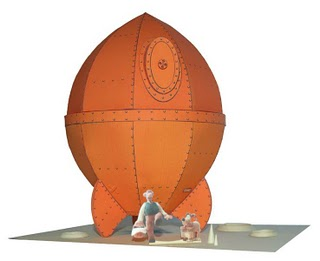
\includegraphics[width=0.45\textwidth]{figures/wallace+and+gromit+rocket+papercraft.jpg}
\caption{Our spaceship.}\label{fig:spaceship}       % Give a unique label
\end{center}
\end{figure}

Cras fringilla libero at sapien dapibus
porta. Maecenas dapibus congue tempor. Aenean et diam lacus, ut
malesuada enim. Integer tristique dictum enim nec
tincidunt. Pellentesque volutpat, neque et euismod pharetra, tortor
augue tincidunt odio, pellentesque mollis nulla diam ac velit. Donec
leo lacus, tempor nec porttitor et, placerat sed eros. Aliquam vel
urna at libero molestie ornare. Morbi quis lectus mi.

Pellentesque volutpat, neque et euismod pharetra, tortor
augue tincidunt odio, pellentesque mollis nulla diam ac velit. Donec
leo lacus, tempor nec porttitor et, placerat sed eros. Aliquam vel
urna at libero molestie ornare. Morbi quis lectus mi.

Etiam fermentum dapibus tristique. Ut mauris lectus, porta vel auctor
ac, hendrerit et sem. Fusce arcu augue, adipiscing fringilla eleifend
in, consequat non orci. Integer non nulla risus. Morbi cursus
condimentum tellus, sit amet suscipit nisl rutrum eget. Sed porttitor
consequat arcu, a religieuse au chocolat pulvinar ut. Class aptent taciti
sociosqu ad litora torquent per conubia nostra, per inceptos
himenaeos. Aenean urna erat, vehicula nec consequat sit amet, pretium
eget enim. Mauris vehicula sagittis nisi tincidunt mattis. Aliquam sed
orci ut orci suscipit suscipit. Morbi iaculis, ligula ac varius
congue, lorem sem vestibulum mi, ut lacinia diam mi eget diam. Ut
gravida convallis nisl, non tincidunt neque luctus vel. Aenean
volutpat blandit imperdiet. Ut feugiat, tellus quis accumsan
tincidunt, sem erat laoreet risus, sit amet dignissim turpis nulla at
elit. Suspendisse sit amet mauris id sapien vehicula placerat. Aliquam
condimentum neque dui, vel suscipit eros.

\begin{figure}[h]
\begin{center}
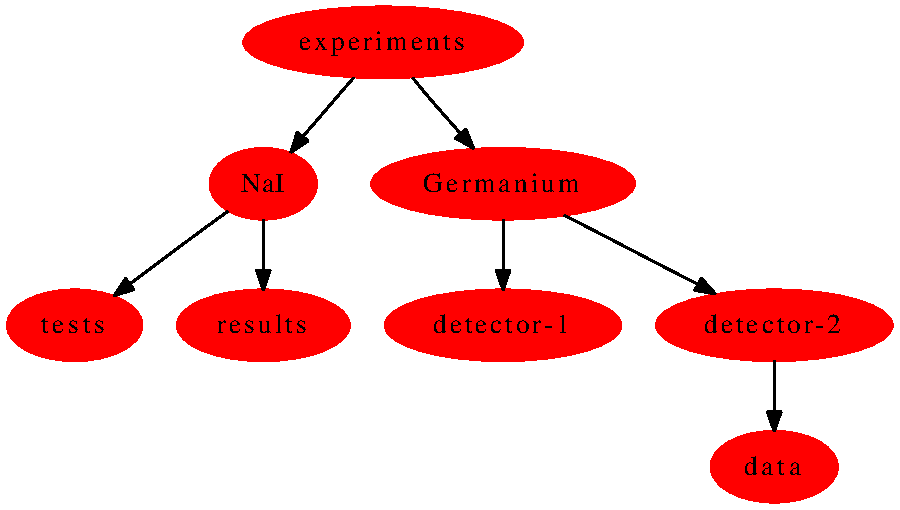
\includegraphics[width=0.45\textwidth]{figures/dirtree.pdf}
\caption{The caption.}\label{fig:spectrum}       % Give a unique label
\end{center}
\end{figure}


\section{Results}
\subsection{Moon is a nice place for a picnic}

Moon is a very nice place to do a Sunday afternoon picnic. Our trip
is described in details in~\cite{trip}.

Etiam fermentum dapibus tristique. Ut mauris lectus, porta vel auctor
ac, hendrerit et sem. Fusce arcu augue, adipiscing fringilla eleifend
in, consequat non orci. Integer non nulla risus. Morbi cursus
condimentum tellus, sit amet suscipit nisl rutrum eget. Sed porttitor
consequat arcu, a pellentesque nunc pulvinar ut. Class aptent taciti
sociosqu ad litora torquent per conubia nostra, per inceptos
himenaeos. Aenean urna erat, vehicula nec consequat sit amet, pretium
eget enim. Mauris vehicula sagittis nisi tincidunt mattis. Aliquam sed
orci ut orci suscipit suscipit. Morbi iaculis, ligula ac varius
congue, lorem sem vestibulum mi, ut lacinia diam mi eget diam. Ut
gravida convallis nisl, non tincidunt neque luctus vel. Aenean
volutpat blandit imperdiet. Ut feugiat, tellus quis accumsan
tincidunt, sem erat laoreet risus, sit amet dignissim turpis nulla at
elit. Suspendisse sit amet mauris id sapien vehicula placerat. Aliquam
condimentum neque dui, vel suscipit eros.

The results are shown in Fig. \ref{fig:picnic}.

\begin{figure}[h]
\begin{center}
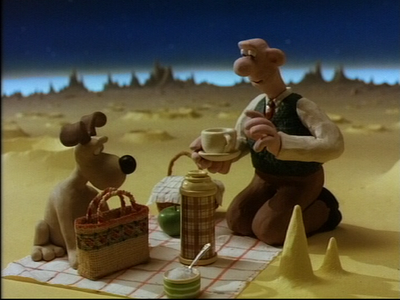
\includegraphics[width=0.45\textwidth]{figures/A_Grand_Day_Out.png}
\caption{Our picnic.}\label{fig:picnic}       % Give a unique label
\end{center}
\end{figure}


\subsection{Moon samples taste good}

On our way back, Gromit and I tasted all the cheese samples collected
from various places on the Moon surface. Our results are given in
Table~\ref{tab:results}. 

Lorem ipsum dolor sit amet, consectetur adipiscing elit. Aenean
consequat sem velit, id ornare quam. Sed in augue mi, a mattis
libero. In sit amet nisl massa. Pellentesque auctor ante non nisl
dictum non molestie neque malesuada. Pellentesque odio arcu, tristique
vel ultricies vitae, vestibulum at enim. Fusce sed ipsum vel tellus
sollicitudin congue quis ac nisl. Duis rutrum eleifend nunc vel
ultrices. Sed vitae dolor at velit ultrices iaculis. Ut blandit, ipsum
sit amet sagittis eleifend, nisi magna ultrices nibh, non tristique
sapien purus in augue. Sed metus leo, mollis vel luctus eu, ultricies
vitae augue. Aliquam auctor luctus euismod. Pellentesque volutpat
vulputate rutrum. Vivamus vel lacus tincidunt libero auctor semper.

\begin{table}[h]
\begin{center}
\begin{tabular}{l|ll}
\hline
\noalign{\smallskip}
Cheese Sample & Test by Wallace &  Test by Gromit \\
\noalign{\smallskip}
\hline
\noalign{\smallskip}
\#1 & Good           & Best \\
\#2 & Quite Good     & Ok \\ 
\#3 & Too many holes & Good \\ 
\noalign{\smallskip}
\hline
\end{tabular}
\caption{Moon cheese sample testing.}\label{tab:results}   % Give a unique label
\end{center}
\end{table}


\section{Discussion}

Etiam fermentum dapibus tristique. Ut mauris lectus, porta vel auctor
ac, hendrerit et sem. Fusce arcu augue, adipiscing fringilla eleifend
in, consequat non orci. Integer non nulla risus. Morbi cursus
condimentum tellus, sit amet suscipit nisl rutrum eget. Sed porttitor
consequat arcu, a pellentesque nunc pulvinar ut. Class aptent taciti
sociosqu ad litora torquent per conubia nostra, per inceptos
himenaeos. Aenean urna erat, vehicula nec consequat sit amet, pretium
eget enim. Mauris vehicula sagittis nisi tincidunt mattis. Aliquam sed
orci ut orci suscipit suscipit. Morbi iaculis, ligula ac varius
congue, lorem sem vestibulum mi, ut lacinia diam mi eget diam. Ut
gravida convallis nisl, un éclair au café non tincidunt neque luctus vel. Aenean
volutpat blandit imperdiet. Ut feugiat, tellus quis accumsan
tincidunt, sem erat laoreet risus, sit amet dignissim turpis nulla at
elit. Suspendisse sit amet mauris id sapien vehicula placerat. Aliquam
condimentum neque dui, vel suscipit eros.

Aenean urna erat, vehicula nec consequat sit amet, pretium eget
enim. Mauris vehicula sagittis nisi tincidunt mattis. Aliquam sed orci
ut orci suscipit suscipit. Morbi iaculis, ligula ac varius congue,
lorem sem vestibulum mi, ut lacinia diam mi eget diam. Ut gravida
convallis nisl, non tincidunt mousse au chocolat neque luctus
vel. Aenean volutpat blandit imperdiet. Ut feugiat, tellus quis
accumsan tincidunt, sem erat laoreet risus, sit amet dignissim turpis
nulla at elit. Suspendisse sit amet mauris id sapien vehicula
placerat. Aliquam condimentum neque dui, vel suscipit eros.

Integer venenatis adipiscing tristique. Vestibulum ullamcorper blandit
tellus, quis suscipit justo ultricies in. Quisque mauris tellus,
viverra ac vestibulum eget, faucibus vitae ipsum.  The main results
are explained in Tab.~\ref{tab:results}.

Nulla nec mauris sit amet tortor commodo sollicitudin sed nec
sem. Praesent in leo in dolor sagittis luctus. Aenean sed nibh elit,
vitae elementum est. Vestibulum sed ultrices orci. Nullam at lorem eu
justo luctus gravida at at sapien. Suspendisse potenti. In a nunc eu
turpis vestibulum convallis. Vestibulum ante ipsum primis in faucibus
orci luctus et ultrices posuere cubilia Curae; Proin non sollicitudin
eros. Vivamus egestas tortor et dui dapibus sed pulvinar nunc
bibendum. Vivamus hendrerit, dolor eu ornare lacinia, ipsum libero
ultricies diam, vitae aliquet tellus dolor vel sem. Sed viverra
fermentum urna, at ultrices urna dapibus et. Fusce posuere justo et
lectus imperdiet fringilla. Etiam feugiat fringilla adipiscing. Sed
interdum magna vitae est luctus quis sollicitudin libero
dapibus. Aliquam erat volutpat.


%
% Non-BibTeX users please use
\begin{thebibliography}{}
%
% and use \bibitem to create references.
%
\bibitem{Boh}A. Bohr and B.R. Mottelson, Nuclear Structure, vol. 2, Benjamin,
New York, 1975.

\bibitem{ipn-web} \url{http://ipnweb.in2p3.fr}

\bibitem{trip} Nick Park, \textsl{A Grand Day Out}, 1989, \url{http://en.wikipedia.org/wiki/A_Grand_Day_Out}

\end{thebibliography}


\end{document}
